\documentclass[12pt]{spieman}  % 12pt font required by SPIE;
%\documentclass[a4paper,12pt]{spieman}  % use this instead for A4 paper
\usepackage{amsmath,amsfonts,amssymb}
\usepackage{graphicx}
\usepackage{setspace}
\usepackage{tocloft}

\title{Out-of-the-box photon counting-based imaging and FLIM using multiscaler}

\author[a]{First Author}
\author[a]{Second Author}
\author[b]{Third Author}
\author[a,b,*]{Fourth Author}
\affil[a]{University Name, Faculty Group, Department, Street Address, City, Country, Postal Code}
\affil[b]{Company Name, Street Address, City, Country, Postal Code}

\renewcommand{\cftdotsep}{\cftnodots}
\cftpagenumbersoff{figure}
\cftpagenumbersoff{table} 
\begin{document} 
\maketitle

\begin{abstract}

\end{abstract}

% Include a list of up to six keywords after the abstract
\keywords{optics, photonics, light, lasers, journal manuscripts, LaTeX template}

% Include email contact information for corresponding author
{\noindent \footnotesize\textbf{*}Fourth author name,  \linkable{myemail@university.edu} }

\begin{spacing}{2}   % use double spacing for rest of manuscript

\section{Introduction}
\label{sect:intro}  % \label{} allows reference to this section

\section{System Setup}
\label{sect:setup}

\begin{figure}
\begin{center}
\begin{tabular}{c}
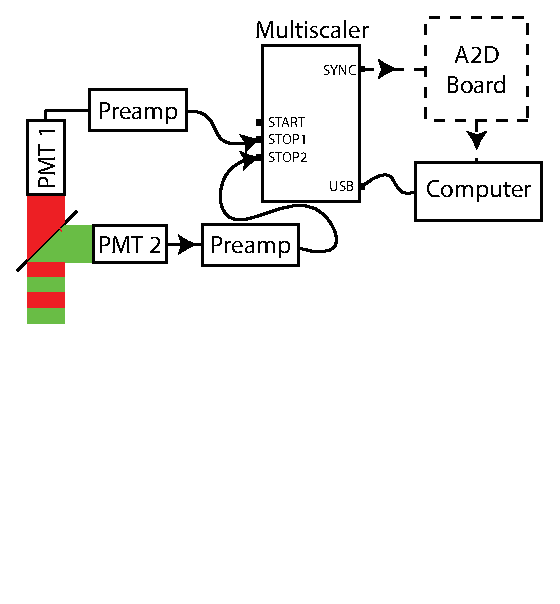
\includegraphics[height=5.5cm]{SystemOutline.eps}
\end{tabular}
\end{center}
\caption 
{ \label{fig:SysOut}
The analog to digital process of the photon counting system.} 
\end{figure} 

\subsection{Correction of galvo ``pixel-shift''}

\section{Results}
\label{sect:results}

\begin{figure}
\caption{FLIM using Multiscaler.}
\end{figure}

\begin{figure}
\caption{Comparison of with or without Rossman \& Grabiner.}
\end{figure}

\begin{figure}
\caption{Online imaging using SYNC OUT}
\end{figure}

\begin{figure}
\caption{Calcium imaging + movies}
\end{figure}

\section{Discussion}
\label{sect:discussion}

\subsection{Caveat: USB 3.0}

\subsection{Caveat: Online imaging}

\subsection{Rossman and Grabiner for regular galvo images}


\appendix    % this command starts appendixes

% \disclosures 
\subsection*{Disclosures}
Conflicts of interest should be declared under a separate header. If the authors have no relevant financial interests in the manuscript and no other potential conflicts of interest to disclose, a statement to this effect should also be included in the manuscript.

\acknowledgments 
This unnumbered section is used to identify those who have aided the authors in understanding or accomplishing the work presented and to acknowledge sources of funding.  

%%%%% References %%%%%

\bibliography{BibPhotonCounting}   % bibliography data in report.bib
\bibliographystyle{spiejour}   % makes bibtex use spiejour.bst

%%%%% Biographies of authors %%%%%

\vspace{2ex}\noindent\textbf{First Author} is an assistant professor at the University of Optical Engineering. He received his BS and MS degrees in physics from the University of Optics in 1985 and 1987, respectively, and his PhD degree in optics from the Institute of Technology in 1991.  He is the author of more than 50 journal papers and has written three book chapters. His current research interests include optical interconnects, holography, and optoelectronic systems. He is a member of SPIE.

\vspace{1ex}
\noindent Biographies and photographs of the other authors are not available.

\listoffigures
\listoftables

\end{spacing}
\end{document}